
\begin{figure}[h]        
    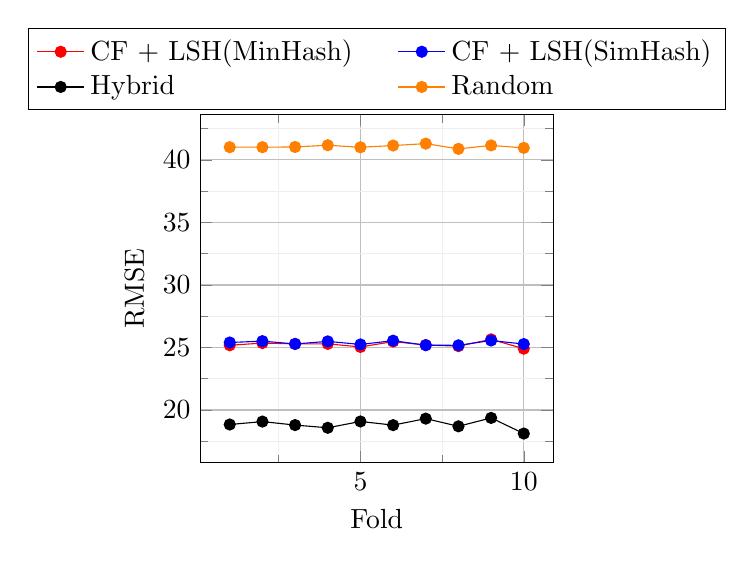
\begin{tikzpicture}
    \begin{axis}[
        xlabel=Fold,
        ylabel=RMSE,
        height=6cm,
        width = 0.5*\textwidth,
        grid = both,
        minor tick num = 1,
        ytick={5,10,15,20,25,30,35,40,45,50},
        major grid style = {lightgray},
        minor grid style = {lightgray!25},
        legend cell align = {left},
        legend columns=2,
        legend style={/tikz/every even column/.append style={column sep=0.5cm}, at={(0.5,1.25)},anchor=north}
    ]
    
    \addplot[color=red,mark=*] coordinates {
        (1,25.178448339353153)
        (2,25.352886564620366)
        (3,25.2888760488129)
        (4,25.291360771693043)
        (5,25.043269655729336)
        (6,25.47261237902709)
        (7,25.194539887462934)
        (8,25.1093334766324)
        (9,25.65084298411703)
        (10,24.903614294515087) 
    };
    
    \addplot[color=blue,mark=*] coordinates {
        (1,25.40101655539042)
        (2,25.50707829498354)
        (3,25.282345944384055)
        (4,25.488182235568754)
        (5,25.243629660988077)
        (6,25.545665842350086)
        (7,25.182059528905363)
        (8,25.17240750330568)
        (9,25.558109387548264)
        (10,25.273546808402592)
    };

    \addplot[color=black,mark=*] coordinates {
        (1,18.839127399224324)
        (2,19.074063798773896)
        (3,18.794608653578774)
        (4,18.577992867330472)
        (5,19.08377099359237)
        (6,18.78992781603451)
        (7,19.310655102258707)
        (8,18.695251412207323)
        (9,19.367127704190807)
        (10,18.115928974573503)
    };

    \addplot[color=orange,mark=*] coordinates {
        (1,41.02070178651229)
        (2,41.02073650592584)
        (3,41.03795148988962)
        (4,41.17712637033412)
        (5,41.012608022837995)
        (6,41.151036886523904)
        (7,41.30366532607506)
        (8,40.885495836401155)
        (9,41.162476830066545)
        (10,40.96403414477042)
    };
    
    \legend{CF + LSH(MinHash), CF + LSH(SimHash), Hybrid, Random}
    \end{axis}
    \end{tikzpicture}
    
    \caption{\normalfont Root means square error measured on different folds of the real dataset.}
    \label{fig:rmse_real}
\end{figure}
